\documentclass[a4paper, 12pt]{article}

\usepackage[T1]{fontenc}
\usepackage[utf8]{inputenc}
\usepackage[spanish, mexico]{babel}
\usepackage[style=mexican]{csquotes}
\usepackage[margin=2cm,top=2cm,includefoot]{geometry}
\usepackage[spanish, ruled, linesnumbered, lined]{algorithm2e}
\usepackage{amsmath, amsfonts, amssymb, amsthm, amsbsy, cancel}
\usepackage{microtype, parskip}
\usepackage{float, graphicx, subcaption}
\usepackage{circuitikz, tikz, pgfplots}
\usepackage{xcolor}
\usepackage{array, booktabs, multicol, multirow, tabularx}
\usepackage{hyperref, url}
\usepackage{siunitx}
\usepackage{tcolorbox}
\usepackage[style=ieee]{biblatex}
%definir el estilo de lapagina
\usepackage{fancyhdr}
%code
\usepackage{listings}
%Referencias
\addbibresource{code/T4.bib}


%variables de color
\definecolor{greenPortada}{HTML}{69A84F}
\definecolor{CabeceraAcero}{HTML}{5DADE2}
\definecolor{Cabeceraverde}{HTML}{008080}
\definecolor{CabeceraTomate}{HTML}{FF4500}



%cabecera
\setlength{\headheight}{40pt}
\pagestyle{fancy}
\fancyhf{}
\renewcommand{\headrulewidth}{3pt}
\renewcommand{\headrule}{\hbox to \headwidth{\color{Cabeceraverde}\leaders\hrule height \headrulewidth\hfill}}

%variables globales

\newcommand{\lineal}{img/lineal.png}
\newcommand{\nolineal}{img/nol.png}
% \newcommand{\}{img/}
% \newcommand{\}{img/}
% \newcommand{\}{img/}
% \newcommand{\}{img}

% \newcommand{\codeA}{code/}
% \newcommand{\codeB}{code/}


%gestion de hipervinculos
\hypersetup{
    breaklinks=true,
    colorlinks=true,
    citecolor=black,
    filecolor=magenta,
    linkcolor=black, 
    urlcolor=cyan
}
%gestor de codigo
\lstset{
    language=Matlab,
    basicstyle=\ttfamily,
    keywordstyle=\color{CabeceraAcero},
    commentstyle=\color{green!50!black},
    stringstyle=\color{CabeceraTomate},
    numbers=left,
    numberstyle=\tiny,
    numbersep=5pt,
    frame=single,
    breaklines=true,
    breakatwhitespace=true,
    tabsize=2
}

%Encabezado
\title{Redes convolucionales}
\author{Universidad Nacional Autónoma de México.\\Facultad de Estudios Superiores Cuatitlán.\\Palomino Alfonso Edgar.\\Vargas Gachuz Alonso}
\date{\today}
\cfoot{\thepage}

\begin{document}
    \maketitle 
    \begin{abstract}      
        El uso de las redes neuronales convolucionales \emph{(RNC)} se da a partir de un mejor manejo de imágenes a través de esta, que haciendo uso de redes neuronales con funciones lineales. Esto en conjunto con la capacidad de cómputo dispuesta en aumento, permiten su implementación, ya que a través de una tarjeta gráfica pequeña pero potente se pudo realizar el procesamiento de 4 imágenes que se etiquetaron pero no se trataron tomando en cuenta un conjunto de datos sin un tratamiento adecuado que si bien es posible encontrarlo en la realidad no es sencillo realizarlo, lo cual puede dificultar la implementación para un proyecto concreto donde, como este caso, se busca responder a casos específicos como señales de activación para un sistema. 
    \end{abstract} 
    \vspace{2ex}

    \section{Introducción.}
    El uso de redes neuronales de funciones lineales limitan las dimensiones o parámetros que se pueden trabajar en conjunto para el diseño de la red neuronal, ya que se busca segmentar la salida a un caso positivo o negativo sobre una línea recta como se puede observar en la figura~\ref{fig:lin}, cosa que se complica al tener más parámetros de entrada para el análisis, este caso se presenta en las imágenes al tener como entradas más de una dimensión para el análisis dejando un sistema mucho más complejo como en la figura~\ref{fig:nolin}, debido a esto es que se plantean las RNC que además de tener diferentes capas de entrada tiene la particularidad de usar redes simples que extraen características particulares cada una, las cuales pasan a otra neurona que agrupa dichas características para determinar un patrón más complejo sobre la imagen, de esta manera es que se pueden reconocer curvas y líneas en conjunto para determinar que algo es una mano o una manzana, este modelo está basado en el sistema de neuronas en la corteza visual primaria de un cerebro biológico. 
    El proceso de extracción de información resulta interesante debido a que en el caso más simple, el cual se representa por un arreglo unidimensional donde se puede extraer el valor de 0 y 1 a valores discretos en el intervalo de 0 a 255, (una escala de grises) se puede obtener un mapa de bits que representa sobre una imagen que valor de blanco o negro se puede obtener algo parecido a el sistema de control difuso, donde no se asigna un valor absoluto del sistema si no que se segmenta sobre una escala y en función de esto se considera una reacción, pero esto representa una limitante, independientemente del color, de que se tiene una posición absoluta del arreglo de bits a identificar, esto genera confusión a las salidas ya que si deslizamos, rotamos, o manipulamos la imagen de alguna manera, esta perderá la coincidencia con dicho mapa, esto como se comentó anteriormente se arregla colocando o centrando la atención de la red sobre patrones básicos (líneas, curvas, etc.) que forman o resultan indispensable sobre la imagen, lo cuales se agrupan para formar un mapa de coincidencia de dichas figuras, de esta manera no importa si el arreglo de bits no coincide, lo que importa es que ciertos patrones estén presente sobre la imagen, además de que a mayor detalle más nutre a la red cosa que sin las RNC no ocurre ya que tener más de una dimensión genera funciones indeterminadas sobre las cuales no se puede obtener una segmentación correcta de los casos donde la salidas son correctas o no, así de esta manera si el color no es indispensable ayuda a tener un patrón de figuras básicas que determina si algo es una manzana o un perro, si además de eso se le agrega los 3 parámetros de color para determinar si una figura redonda es una uva, un coco o un melón, la red es más precisa al tener más detalles, pero estop requiere un data de mayor tamaño, esto con el fin de adecuar la RNC para que funcione de la mejor manera. 

    \begin{figure}[H]
        \centering
        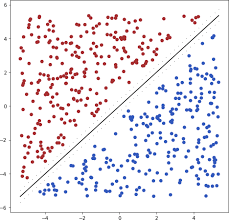
\includegraphics[width=0.4 \linewidth]{\lineal}
        \caption{Conjunto separable linealmente}
        \label{fig:lin}
    \end{figure}

    \begin{figure}[H]
        \centering
        \includegraphics[width=0.4 \linewidth]{\nolineal}
        \caption{Conjunto no separable de manera lineal}
        \label{fig:nolin}
    \end{figure}

    \section{Estado del arte.}
    La redes convolucionales han tenido una gran auge, ya que pesar de que la teoría de la relación entre el procesamiento de datos de un cerebro biológico y su homologación con el procesamiento de datos por un microprocesador se tenía claro que no existe comparación ya que hay una cantidada mucho mayor de neuronas en un cerebro biológico que microprocesadores en una computadora actual, pero los procesadores cuentan con la capacidada de poseer mayor velocidad ya que como menciona A. Moreno en su tesis el valor de este procesamiento en los humanos es de milisegundo mientras que en la electrónica moderna es de nanosegundos, cosa que brinda una ventaja palpable en el hecho de necesitar poco más de un siglo entre la propuesta de las teorías de estudio del trabajo pionero de Ramón y Cajal en la disertación de la neurona, además de poder hacer énfasis en que fue aún menos tiempo entre las propuestas de Hubel y Wiesel acerca de la corteza visual para tener propuestas y algoritmos que trabajan con el hardware actual para realizar dichas tareas, cosa que puede dejarse ver a través de la historia tomo menos tiempo la evolución de aquellas partes biológicas que estos algoritmos aplicables\cite{artola2019clasificacion}.\\
    Si bien esto es palpable debido a este tiempo dimensionado, el artículo de optimización distribuida de redes convolucionales para la clasificación de las imágenes no deja cabida para la duda, ya que su visión de la optimización de RNC distribuidas consta de tener más de una sola computadora dedicada a una sola tarea teniendo un organigrama de principal y secundarios (maestro y esclavos), con el cual logra sacar porcentajes de precisión iguales o mayores a otras arquitecturas propuestas, teniendo en consideración de que el tiempo se reduce al colocar más máquinas dedicadas a la tarea, dejando claro que a mayor cantidada de neuronas el algoritmo puede trabajar de mejor manera, lo cual hace el contraste con todo lo anteriormente dicho\cite{hernandez2019optimizacion}\\
    En general lo citado hasta ahora deja de manera clara y básica todo los conceptos necesarios para poder trabajar con RNC, pero el informe de proyecto de grado denominado redes neuronales convolucionales aplicadas a demosaicing y denoising, detalla a profundidad todos los conceptos utilizados, estos nos permite entender de una manera más formal todo aquello se tomará en la sección de conocimientos previos además de proporcionar detalles acerca de cómo es que las imágenes digitales son procesadas para su obtención digital, que aunque como se hace notar en dicho informe todos los fabricantes son libre de llevar a cabo estos  procesos tener un panorama general nos permite comprender el procesamiento de imágenes así como los componentes que se procesan y el porqué de los diferentes tratamiento que le daremos a las imágenes una vez estemos implementado la RNC para el reconocimiento patrones sobre diferentes imágenes digitales y que de ser el caso las componentes de color que se requieren para un mejro desempeno de la RNC\cite{balduvin2019redes}

    %conocimientosP
    \section{Conocimientos previos.}
    El valor de las RNC está en procesar en paralelo las características de una imagen sin depender de la información que esta proporciona, si bien el orden de dichos valores es importante para el color ya que se utiliza un sistema RGB, el resto de la imagen depende más de la figuras propias del objeto que la RNC pueda identificar para determinara patrones claves que realizan la coincidencia de una imagen con su etiqueta.

    \subsection{Perceptron.}
    El perceptrón puede definirse como la función matemática que simula la unidad más básica del pensamiento del ser humano la cual cuenta con entradas, pesos sinápticos, desviaciones y salidas, la cual pondera el valor de cada entrada en función del valor del peso sináptico que se proporciona a dicha entrada, sumada a la desviación de la neurona genera la salida para la decisión final, se puede tener múltiples perceptrones juntos, lo que conforma la redes neuronales densas que como en el nombre se puede percibir es un cúmulo de perceptrones interconectados entre sí para generar un comportamiento en la salida parecido a las decisiones humanas. Dicho comportamiento se define con la función matemática siguiente:
    \[
    f(x) =
    \begin{cases}
        0 & \text{si } \sum\limits_{1}^{m} w_i x_i + b < z, \\
        1 & \text{en otro caso}.
    \end{cases}
    \]
    Donde $m$ es la cantidad de entradas , $xi$ es el valor de la entrada $i$, $b$ corresponde al valor de la desviación asignado a la neurona y $wi$ corresponde al coeficiente $i$ de la transformación lineal antes mencionada correspondiente al peso sináptico asignado a la entrada $i$. Por último $z$ queda acotado dentro de la función de activación.\\
    Debe hacerse notar que es una transformación lineal, lo cual determina que solo podamos hacer uso de dicho perceptrón en conjuntos que sean linealmente separables, en caso contrario las salidas generan errores al no poder hacer una división clara entre los datos.

    \subsection{Aprendizaje profundo.}
    El deep learning es un subconjunto de algoritmos pertenecientes al machine learning el cual se diferencia en el tipo de datos que se procesan para su entrenamiento ya que mientras el machine learning utiliza datos estructurados y clasificado para determinar las salidas, el deep learning no requiere dicha estructuración lo que permite trabajar con imágenes de una manera menos compleja ya que no tenemos que estructurara y dar un sentido de cada dato que ingresa si no que el propio algoritmo determina cuales son los datos que importan para procesarlos para de esta manera llegar a la misma salida con la precisión de predicción adecuada sin haber dado la estructuración a cada dato, entiéndase como dato la información de una imagen procesada, esto tiene que ver con la parte de que no se requiere determinar un mapa de bits concreto, si no que a través del proceso se determina cierta cantidad de bits en conjunto dentro de los mapas que son relevantes para determinar dicho objeto. 

    \subsection{Convolución.}
    La convolución se refiere al proceso matemático de pasar una matriz núcleo que sirve como filtro para extraer datos de un arreglo matricial, es decir es la operación matemática de un arreglo matricial influido por otro, de esta manera podemos pasar los valores del mapa de bits, por un núcleo de mxn valores que altera el valor de todo el arreglo que dicho de esa manera no genera impacto por eso se toma la referencia de filtro, al cambiar el valor de todo el arreglo se puede tomar que se genera otra imagen en base a la imagen original ( se aplica un filtro) afectando los parámetros de dicha imagen, esto ayuda extraer información de los patrones ya que revisamos valores en conjunto y no solo un arreglo de una dimensión en cada iteración, dicho núcleo a través de la convolución del mapa original generará diferentes salidas lo que permite descomponer una imagen compleja en patrones simples, ya que cada uno de los núcleos y cada convolución generará una imagen diferente de salida o mapa de bits distinto de las cuales la red neuronal debe aprender, de esta manera es como se extraen patrones de relevancia para una imagen, también se puede agregar que es el motivo por el que necesitamos data set grades para entrenar una RNC. 

    \subsection{Funciones de activación comunes.}
    Las funciones de activación pueden ser variadas, pero como siempre se utilizan más unas que otras aquí se colocan 2 de las más usadas, debido a su propiedades todo dependerá de que es lo que buscamos al usar cada una de ellas, ya que modifican el valor de la salida gracias a su comportamiento.
    \begin{itemize}
    \item La función softmax (función exponencial normalizada) es una generalización de la función sigmoidea las cuales una de las funciones de activación más conocidas cuando se trata de redes neuronales, la función Sigmoide introduce un grado de no linealidad a las neuronas de la red. Una función sigmoide es monótona creciente y representa asíntotas en ambos extremos en un valor finito, de esta manera la función Softmax se utiliza como función de activación de salida para la clasificación multiclase porque escala las entradas precedentes de un rango entre el intervalo de $[0,1]$ y normaliza la capa de salida, de modo que la suma de todas las neuronas de salida sea igual a la unidad, debido a la propiedad de la sigmoide y la acotación realizada en la softmax se tiene una función que trabaja con valores más acorde a la normalización de los datos que se hace cada vez que se tratan.
    \item La unidad lineal rectificada, del inglés Rectified Linear Unit (ReLu) es la función de activación más utilizada en los modelos de aprendizaje profundo, debido a que la función devuelve 0 si recibe una entrada negativa, pero para cualquier valor positivo devuelve ese valor, s extremadamente simple de definir y computar, la función ReLU se expresa de la siguiente forma:
    \[
    f(x) =
    \begin{cases}
        0 & \text{si } x\leq 0\\
        x & \text{en otro caso}.
    \end{cases}
    \]
    Donde $z$ es un valor arbitrario. Variantes de ReLU permiten que la red modifique z en tiempo de entrenamiento  
    \end{itemize}

    \subsection{Propagación.}
    La propagación de los datos se da de una manera típica con un forward, que es decir comienza por la entrada y van hacia la salida ( de adelante hacia atrás), durante este proceso se realizan las operaciones correspondientes como son la convolución, el agrupamiento, se usan las funciones de activación y se determina la salida óptima para el sistema, pero durante la fase de entrenamiento se pueda hacer uso de un algoritmo que mejora los resultados obtenidos a través de la optimización del tiempo empleado que es la propagación hacia atrás o back propagation\\
    La propagación hacia atrás es un algoritmo es vital para el entrenamiento de redes neuronales profundas (con más de una capa de neuronas interna), y consiste en propagar el gradiente de la función de costo hacia atrás, actualizando los pesos de cada neurona.\\
    La propagación hacia atrás permite ayudar a corregir los pesos actuales de la red, minimizando el error que comete en un conjunto de ejemplos de entrenamiento. Para lograr esto es necesario conocer el gradiente de la función de activación de cada unidad de cada capa. El algoritmo calcula iterativamente para cada capa estos gradientes, tomando como entrada los gradientes calculados para la capa inmediatamente siguiente, esto nos permite tener una “etapa” dedicada a corregir los errores que cada proceso que la red ha cometido, con lo que el siguiente forward tendrá menos errores.\\
    Realizando un análisis de este proceso, generamos un entrenamiento con errores gracias a él forward, corregimos los errores en función del peso de la culpa que tiene cada etapa de la red, también se minimiza el error gracias a la propagación hacia atrás, lo cual en el proceso ajusta dichos pesos dejando la lista para que se vuelvan a realizar un forward e iterar de esta manera cada época de la RNC. Haciendo una comparación con los algoritmos genéticos donde escogemos la red que queremos que herede sus genes a la siguiente generación, el algoritmo de backpropagation realiza la elección de los pesos que queremos que pases a el siguiente entrenamiento en función de que tanto error han generado o no, si el error es grande la propagación hacia atrás realizará los cambios de los pesos lo que impedirá que dichos errores se lleven a la siguiente época de entrenamiento.

    \subsection{Capas.}
    \subsection{Ajuste.}
    \subsection{Librerias}

    \section{Metodología.}

    \section{Análisis de resultados.}

    \section{Conclusión}
    \printbibliography

\end{document}


    % \begin{equation}
    %     A = \{ ( x,\mu_{A(x)} )/x \in X \}
    % \end{equation}
    % Donde $\mu_{A(x)}$ es una función de pertenencia cuya etiqueta es A y su dominio es $x$
    .
    % \begin{figure}[H]
    %     \centering
    %     \includegraphics[width=0.8 \linewidth]{\conjuntoD}
    %     \caption{Conjuntos difusos}
    %     \label{fig:conjuntoD}
    % \end{figure}

    %\clearpage
    % \lstinputlisting[caption={Ejemplo de código MATLAB.}, label=lst:fis, title={ código 1 : Archivo del sistema de control difuso Mamdani}]{\codeB}

    % \begin{figure}[H]
    %     \centering
    %     \begin{subfigure}{0.8\linewidth}
    %         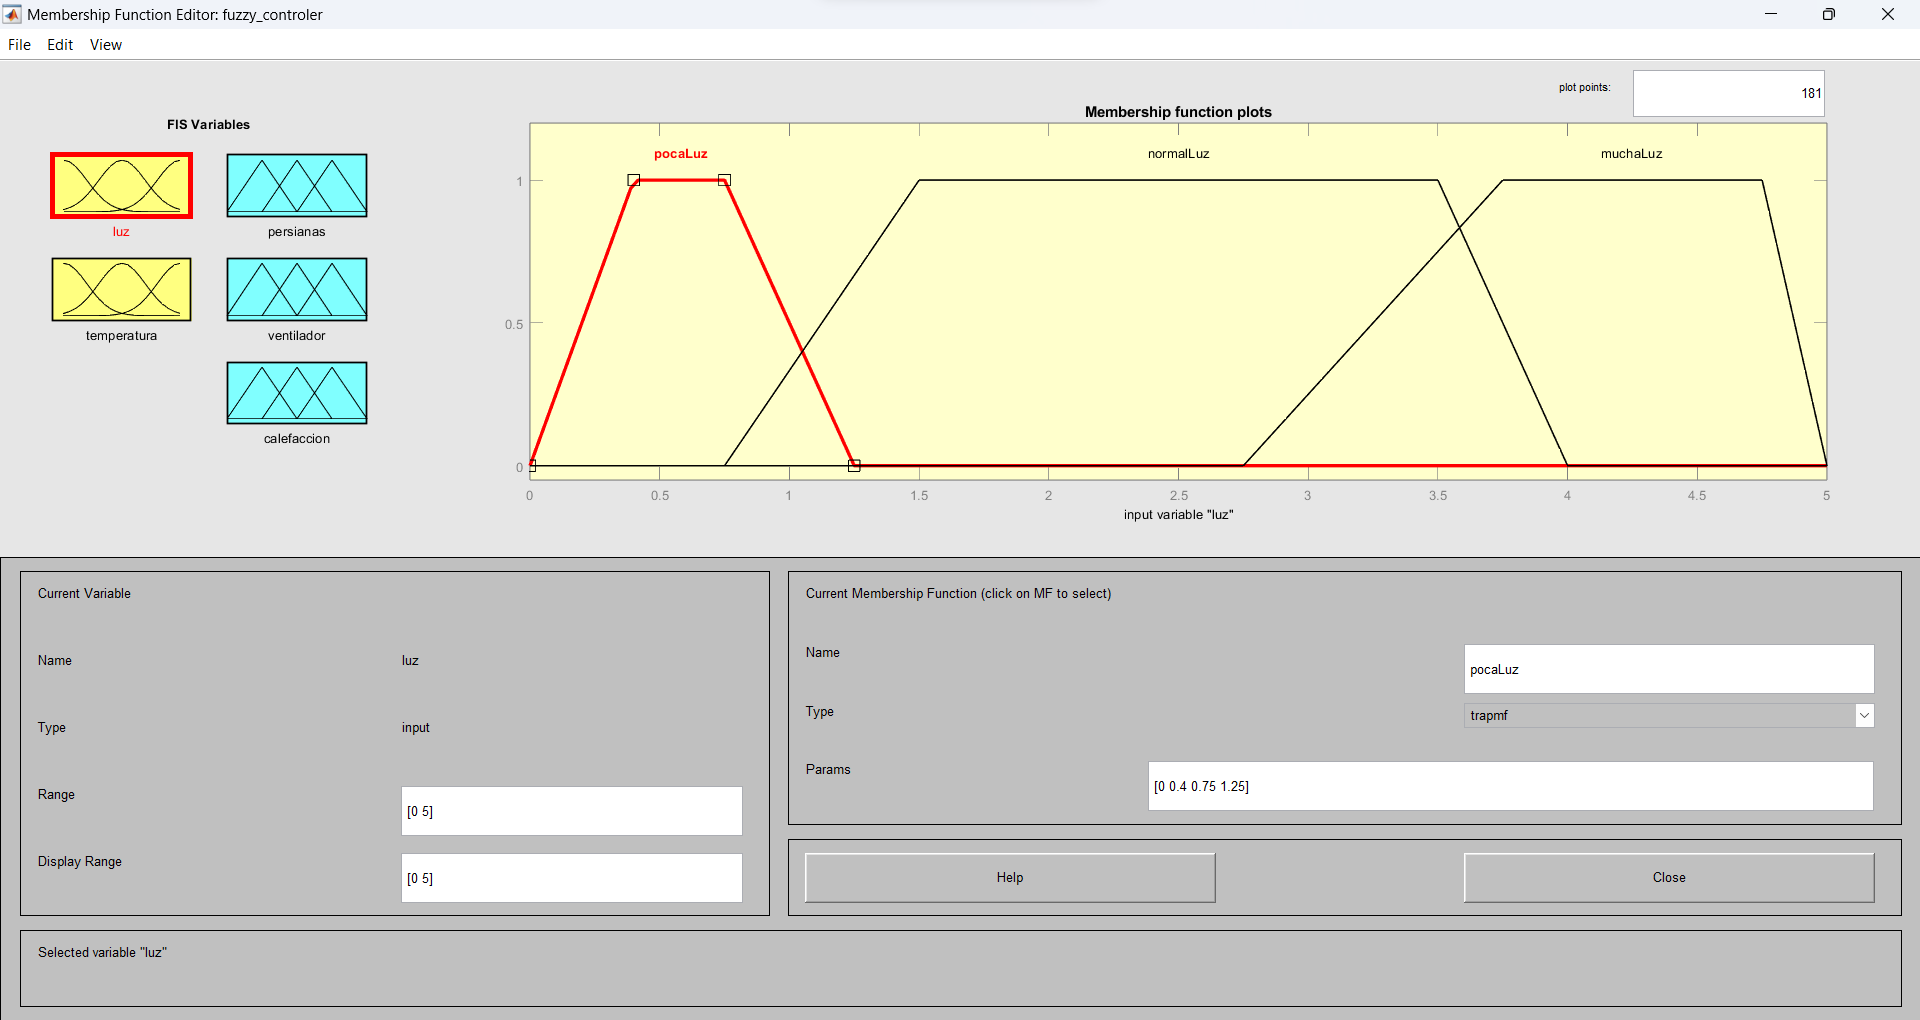
\includegraphics[width=\linewidth]{\luz}
    %         \caption{Conjunto difuso luz}
    %         \label{sub:luz}
    %     \end{subfigure}
    %     \begin{subfigure}{0.8\linewidth}
    %         \includegraphics[width=\linewidth]{\temperatura}
    %         \caption{Conjunto difuso temperatura}
    %         \label{sub:temp}
    %     \end{subfigure}
    %     \caption{Entradas}
    %     \label{fig:nter}
    % \end{figure}